
\chapter{REQUIREMENT ANALYSIS}

\section{\normalsize{\textbf{Requirement analysis}}} 
\subsection{\normalsize{Product Functions}}
\begin{itemize}
\item Query Image
\item Facial Attributes Detection
\item Sparse Code Generator
\item Binary Signature Generation
\item Inverted Indexing
\item Ranking of Resultant Images for Query Image
\item Space complexity Reduces
\item Better performance
\end{itemize}
\subsection{\normalsize{User Classes and Characteristics}}
\textbf{Crime investigation:} 
The Propose System can be use effectively for Criminals identification. Attribute detection from Query Criminal image will retrieve the corresponding matches for Query Image.
\newline \textbf{Medical:}
Medical science can often make excellent use of technologies from other fields. For example, knowledge from automatic facial recognition can also be used for medical analysis of images of organs.
\subsection{\normalsize{Operating Environment}}
\textbf{Hardware Requirement:}
\begin{itemize}
\item 2.80GHz Intel Pentium Processor (min)
\end{itemize}
\textbf{Software Requirement:}
\begin{itemize}
\item Microsoft Windows X P/7(OS)
\item Microsoft V isual S tudio2010
\end{itemize}
\textbf{Dataset:}
\begin{itemize}
\item LFW
\item PubFig
\end{itemize}
\subsection{\normalsize{Design and Implementation Constraints}}
The Propose System will provide Ranking for Query Image with the use of Inverted Indexing but on the behalf of this constraint for Propose System is:
\begin{itemize}
\item Multiple Faces Image will be Rank According to Face Landmark Detection.
\item Query Image should contain Face.
\end{itemize}
\subsection{\normalsize{User Documentation}}
The product will be deploy along with the user manual for the proper guidance to install the software and the tutorials for effectively using various functions provided by the software.
\newpage
\section{\normalsize{\textbf{Project plan}}}
\begin{figure}[ht!]
	\centering
		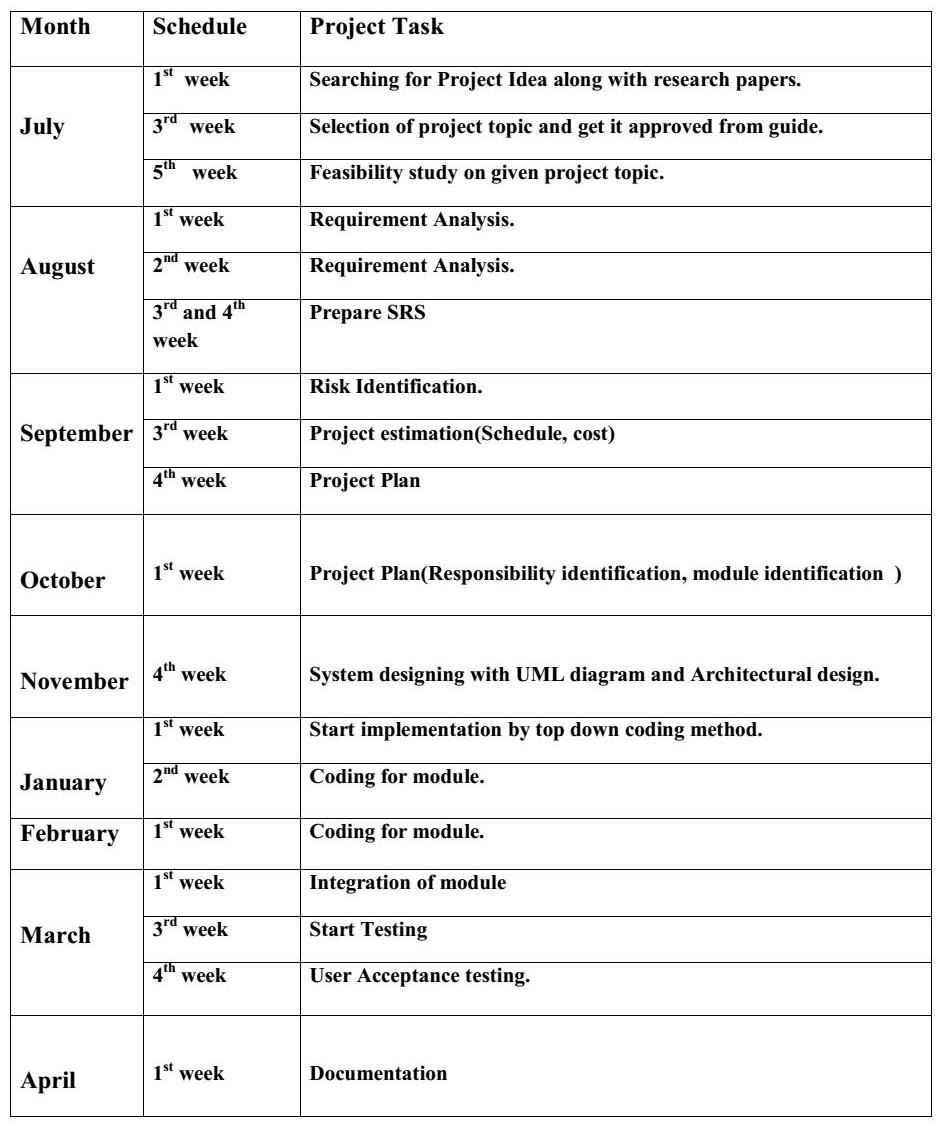
\includegraphics[width=100mm]{plan.jpg}
	\caption{Plan for Project}
	\label{fig:plan}
\end{figure}
\section{\normalsize{\textbf{Team structure}}} 
\begin{table}[h]
\label{sch}
\begin{center}
\begin{tabular}{|c|c|c|c|c|} \hline
		\bfseries Sr.No. & \bfseries Name & \bfseries Task \\ \hline
    \bfseries 1 & Amruta Kumbhakarn &  Coding, Testing \\ \hline
		\bfseries 2 & Sana Mirza &  Documentation, Testing  \\ \hline
		\bfseries 3 & Nikhil Wagh & Coding, Testing  \\ \hline
		\bfseries 4 & Sagar Katarnaware & GUI, Testing  \\ \hline
\end{tabular}
\end{center}
\caption {Team structures.}
\end{table}




%%% Local Variables: 
%%% mode: latex
%%% TeX-master: "../mainrep"
%%% End: 
